\documentclass[sn-basic]{sn-jnl}% Default

% \documentclass[default,lineno,sn-basic]{sn-jnl}% Default
% \documentclass[default,iicol]{sn-jnl}% Default with double column layout

\usepackage{graphicx}%
\usepackage{multirow}%
\usepackage{amsmath,amssymb,amsfonts}%
\usepackage{amsthm}%
\usepackage{mathrsfs}%
\usepackage[title]{appendix}%
\usepackage{xcolor}%
\usepackage{textcomp}%
\usepackage{manyfoot}%
\usepackage{booktabs}%
\usepackage{algorithm}%
\usepackage{algorithmicx}%
\usepackage{algpseudocode}%
\usepackage{listings}%


%% as per the requirement new theorem styles can be included as shown below

\newtheorem{theorem}{Theorem}%  meant for continuous numbers
%%\newtheorem{theorem}{Theorem}[section]% meant for section wise numbers
%% optional argument [theorem] produces theorem numbering sequence instead of independent numbers for Proposition
\newtheorem{proposition}[theorem]{Proposition}% 
%%\newtheorem{proposition}{Proposition}% to get separate numbers for theorem and proposition etc.

\newtheorem{example}{Example}%
\newtheorem{remark}{Remark}%

\newtheorem{definition}{Definition}%

\raggedbottom
%%\unnumbered% uncomment this for unnumbered level heads

\begin{document}

\title[Article Title]{Area-Throughput Efficient Implementations of CRAFT Cipher For Internet of Vehicles - v1.8.0}

\author[1,2]{\fnm{Jiahao} \sur{Xiang}}\email{simple.xjh@qq.com}
\author*[1,2]{\fnm{Lang} \sur{Li}}\email{lilang911@126.com}

\affil*[1]{\orgdiv{College of Computer Science and Technology}, \orgname{Hengyang Normal University}, \orgaddress{\city{Hengyang}, \postcode{421002},  \country{China}}}

\affil[2]{\orgdiv{Hunan Provincial Key Laboratory of Intelligent Information Processing and Application}, \orgname{Hengyang Normal University}, \orgaddress{ \city{Hengyang}, \postcode{421002}, \country{China}}}

\abstract{
    \textbf{Purpose:} With extraordinary growth in the Internet of Vehicles (IoV), the amount of data exchanged between IoV devices is growing at an unprecedented scale.
    Most of the IoV devices need instant response and real-time security to ensure the safety of users.
    The CRAFT cipher that is a lightweight block cipher for low-area can be used in IoV devices.
    In order to better adapt to these environment, the objective of this paper is to explore opportunities to optimize area and throughput for CRAFT cipher targeted for low-resource IoV devices.
    \textbf{Methods:} A novel compact CRAFT implementation is proposed in serialized fashion to achieve a small hardware footprint.
    We propose novel unrolled structure of CRAFT cipher for the high throughput feature.
    \textbf{Results:}The results on Artix-7 show that ...
    \textbf{Conclusion:} Hence, our works let CRAFT cipher more suitable for IoV devices.
}

\keywords{Lightweight block cipher, Internet of Vehicles, Field-programmable gate array(FPGA), Low-area, High-throughput}


\maketitle

\section{Introduction}\label{sec1}

Internet of Vehicles (IoV) is an emerging concept in intelligent transportation systems (ITS) to enhance the existing capabilities of VANETs by integrating with the Internet of Things (IoT) \cite{sharma2019survey}.
As IoT technology continues to advance, IoV technology is also making great progress.
But the same security issues that exist in IoT are also were introduced into IoV.
At the some time, IoV involves a huge amount of dynamic real-time critical data so its security is a major concern.

Lightweight cryptography is a subfield of cryptography that aims to provide solutions tailored for resource-constrained devices \cite{mckay2016report}.
It can provides security with low resource consumption and low delay in IoV environment.

In this work, we propose the three architectures of FPGA implementations for the CRAFT \cite{beierle2019craft}, respectively Round based, Serial, and Loop unrolled.
This allows IoV practitioners to select the architectures that best suit their needs.
The contributions of this article can be summarized as follows.

The rest of this article is organized as follows.
Section~\ref{sec2} presents specification of CRAFT; the proposed the three architectures of FPGA implementations for the CRAFT are present in Section 3; Section 4 presents the implementation results, analysis, and comparison with other similar works; finally, the work is concluded in Section 5.


\section{Specification of CRAFT}\label{sec2}

All notations used in this paper are shown in Table~\ref{tab1}.
CRAFT is a lightweight tweakable block cipher made out of involutory building blocks.
It consists of a 64-bit block, a 128-bit key, and a 64-bit tweak. In this cipher, a 64-bit input plaintext P is transformed into a 64-bit output ciphertext C using a 128-bit key K and a 64-bit tweak T. Figure~\ref{fig1} shows the structure of CRAFT.

\begin{table}[h]
    \caption{Notations used in this paper}\label{tab1}%
    \begin{tabular*}{\textwidth}{@{\extracolsep\fill}lcccccc}
        \toprule
        Notation   & Description                                 \\
        \midrule
        $TK$       & 64-bit tweakeys                             \\
        $RC_i$     & 64-bit round constant in the $i^{th}$ round \\
        $R_i,R'_i$ & Round function                              \\
        $\oplus$   & Bit-wise sum (XOR)                          \\
        \botrule
    \end{tabular*}
\end{table}

\begin{figure}[h]%
    \centering
    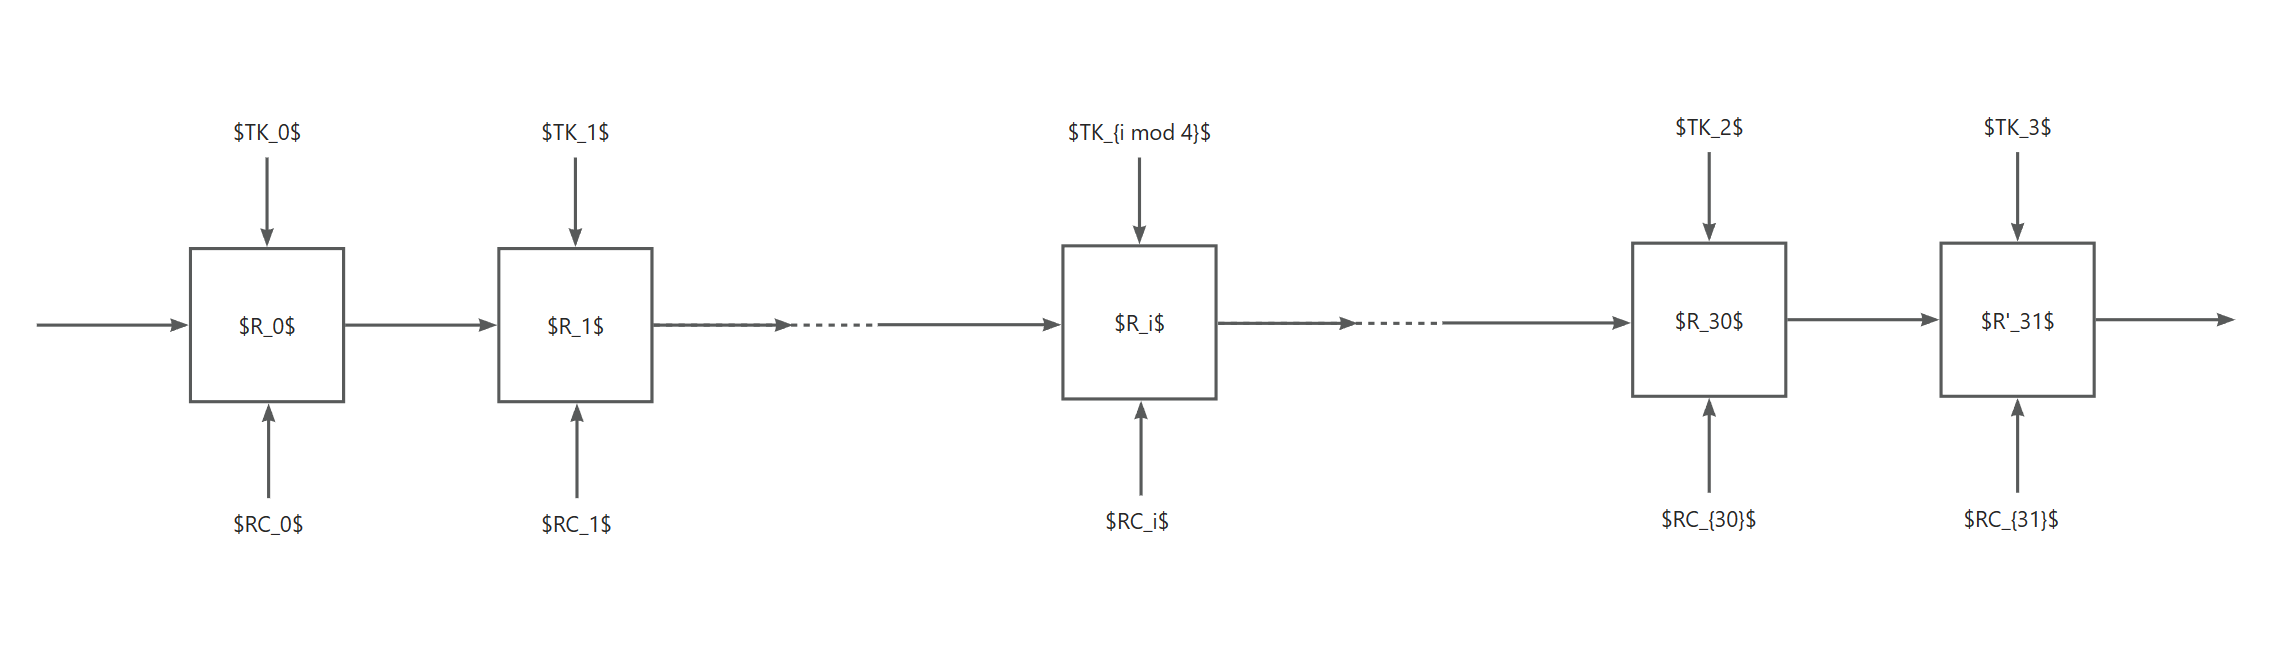
\includegraphics[width=\textwidth]{struct_of_craft.png}   
    \caption{Structure of CRAFT}\label{fig1}
\end{figure}


\section{Proposed Architecture}\label{sec3}

In order to achieve efficient area and throughput, we optimize the components of craft for the first time and propose three implementation architectures, respectively Round based, Serial, and Loop unrolled.

\subsection{Round Based Architecture(A1)}\label{subsec1}
While no FPGA implementation of the round-based architecture is provided in \cite{beierle2019craft}, we have taken the initiative to implement the architecture presented therein for the first time.
Figure~\ref{fig2} is Round-based design architecture of CRAFT.

\begin{figure}[h]%   
    \centering
    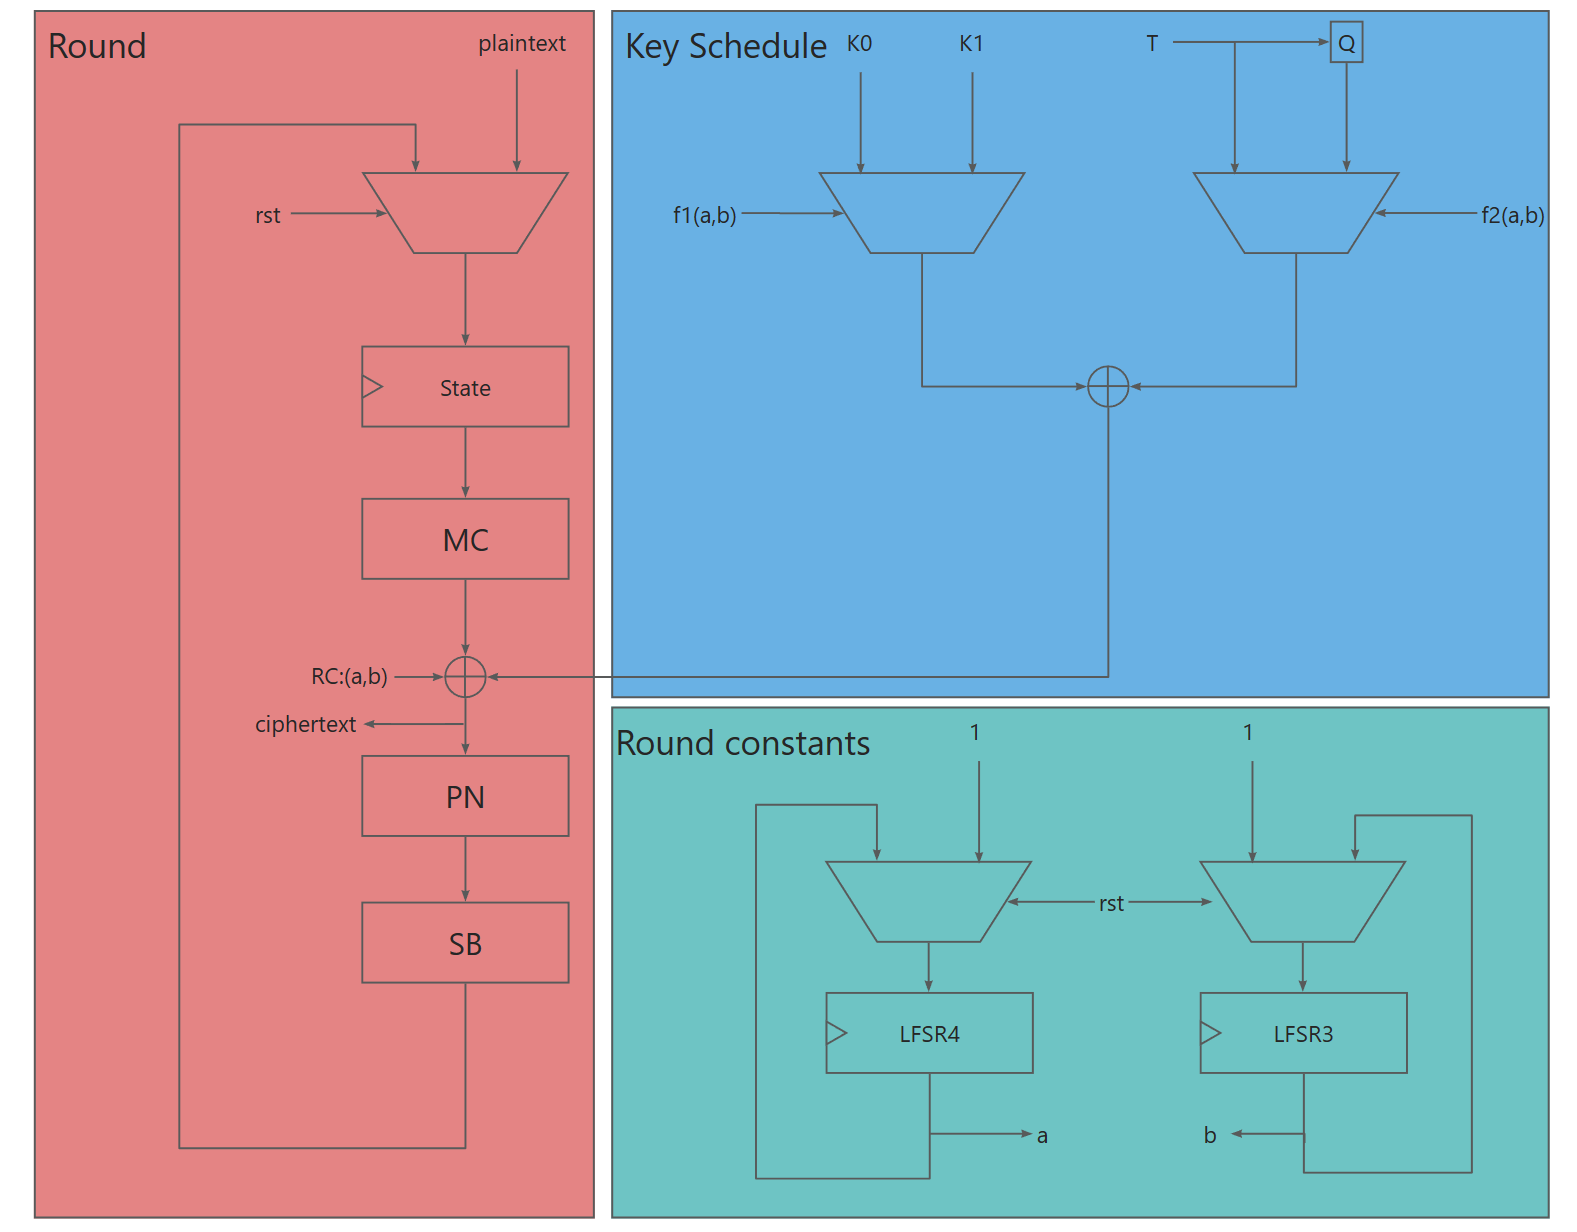
\includegraphics[width=\textwidth]{round_based_design.png}
    \caption{Structure of CRAFT}\label{fig2}
\end{figure}


\subsection{Serial Architecture(A2)}\label{subsec2}
Compared to round-based architecture, serial architecture are able to reuse components and significantly reduce area usage, e.g., the number of S-box is reduced from 16 to 1.
The clock gating technique is also used to enable each component and reduce the energy consumption of encryption. Our proposed architecture is presented in Figure~\ref{fig3}.
The design includes one Sub-Box, one 4-bit Mix-columns, two register banks for storing keys (called Key-Register) and plaintext (called State-Register), which also act as temporary registers for storing the intermediate results.
In order to store intermediate results into State-Register bank, the design has one feedback paths.
PermuteNibbles is included in State-Register bank.
It is noticeable that since the execution of permute requires 64-bit, in order to reuse the State-Register block, we change the order of execution of Sub-Box and Permute.
And the first round of encryption process through the control signal to avoid Permute operation, to ensure the correctness of the encryption algorithm.

\begin{figure}[h]%   
    \centering
    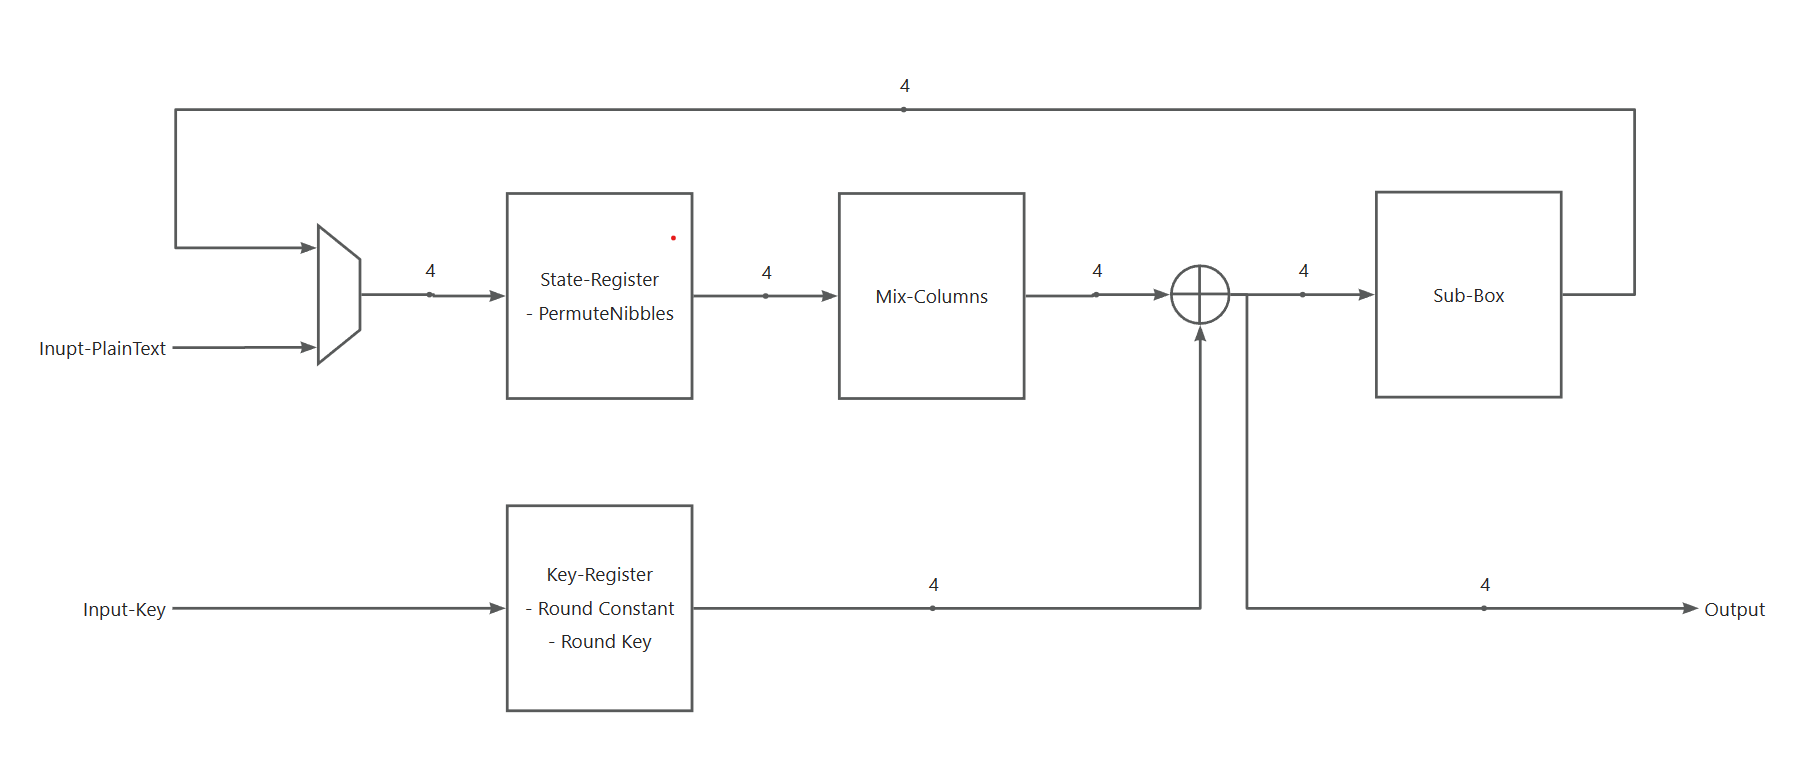
\includegraphics[width=\textwidth]{serial_design.png}
    \caption{Serial architecture of CRAFT}\label{fig3}
\end{figure}


\subsubsection{Sub-Box Optimization }\label{subsubsec1}
Sub Box provides a confusing characteristic for the entire encryption algorithm, however it requires a large amount of area.
There are different methods of implementation of Sub Box.
The most popular implementation is using a lookup table (LUT), such as \cite{lara2017lightweight}.
However it uses a lot of flip-flop, which will bring a lot of area consumption.
Using S-Box's equivalent logical expression for this will reduce area consumption, such as \cite{bao2019peigen}, \cite{bib16}.

SAT solvers can be used to find S-Box that satisfy certain implement, such as being resistant to software or hardware implement.
In more detail, the S-Box implement can be encoded as Boolean constraints by representing the S-Box as a truth table and then using Boolean variables to represent the input and output bits of the S-Box.
The constraints can then be formulated based on the desired implement of the S-Box.
Once the S-Box implement are encoded as Boolean constraints, a SAT solver can be used to find a satisfying assignment to these constraints, which corresponds to an S-Box that satisfies the desired implement.

The gate equivalent complexity(GEC) of a SAT instance is the number of logical gates required to implement the Boolean formula that represents the instance.
GEC can be calculated by converting the Boolean formula into a circuit of logical gates, such as AND, OR, and NOT gates.
The number of gates in the circuit corresponds to the GEC of the instance.

In our design, we optimize and use GEC encoding scheme of \cite{bib16} to implement the S-Box.
Our encoding scheme as follows in Equation~\ref{eq1}:

\begin{align}
    \forall i \in \{0,1,\ldots ,K-1\}: \nonumber                                                                  \\
    T_i & = F_{if} (BB_i[0], \thicksim (Q_{4i} \cdot Q_{4i+1}) \cdot \thicksim Q_{4i+2} \cdot Q_{4i+3}) \nonumber \\
        & \quad + F_{if} (BB_i[1], Q_{4i+2} \cdot (Q_{4i} + Q_{4i+1})) \nonumber                                  \\
        & \quad + F_{if} (BB_i[2], Q_{4i} \cdot Q_{4i+1} \cdot Q_{4i+2}) \nonumber                                \\
        & \quad + F_{if} (BB_i[3], Q_{4i+2}) + F_{if} (BB_i[4], Q_{4i}) \nonumber                                 \\
        & \quad + F_{if} (BB_i[5], Q_{4i} \cdot Q_{4i+1}) \nonumber                                               \\
        & \quad + F_{if} (BB_i[6], Q_{4i} + Q_{4i+1}) + F_{if} (BB_i[7], \max). \label{eq1}
\end{align}

where $K$ is numbers of the logical gates, $Q_{4i}-Q_{4i+3}$ is the input of the $i^{th}$ logical gate, $T_i$ is the output of the $i^{th}$ logical gate, and $F_{if}$ is a function that returns the value of the second argument if the first argument is true and returns the value of zero otherwise.
The value of $max$ is all one's in the binary expression, which is represented logically as an inverse.
$BB_i$ represents the type of the $i^{th}$ logical gate, which is a 8-bit binary number. The different types of logical gate used in this encoding scheme are listed in Table~\ref{tab3}.


\begin{table}[h]
    \caption{Encoding of different types of logical gate}\label{tab3}%
    \begin{tabular*}{\textwidth}{@{\extracolsep\fill}lcccccc}
        \toprule
        logical expression & $BB_i$[0:7] & gate type \\
        \midrule
        $Q_0 \oplus Q_1$ & 0 0 0 0 0 0 1 0 & XOR \\
        $\sim (Q_0 \oplus Q_1)$ & 0 0 0 0 0 0 1 1 & XNOR \\
        $Q_0 \land Q_1$ & 0 0 0 0 0 1 0 0 & AND \\
        $\sim (Q_0 \land Q_1)$ & 0 0 0 0 0 1 0 1 & NAND \\
        $Q_0 \lor Q_1$ & 0 0 0 0 0 1 1 0 & OR \\
        $\sim (Q_0 \lor Q_1)$ & 0 0 0 0 0 1 1 1 & NOR \\
        $\sim Q_0$ & 0 0 0 0 1 0 0 1 & NOT \\
        $\sim Q_1$ & 0 0 0 0 1 0 1 1 & NOT \\
        $\sim Q_2$ & 0 0 0 1 0 0 0 1 & NOT \\
        $Q_0 \oplus Q_1 \oplus Q_2$ & 0 0 0 1 0 0 1 0 & XOR3 \\
        $\sim (Q_0 \oplus Q_1 \oplus Q_2)$ & 0 0 0 1 0 0 1 1 & XNOR3 \\
        $Q_0 \land Q_1 \land Q_2$ & 0 0 1 0 0 0 0 0 & AND3 \\
        $\sim (Q_0 \land Q_1 \land Q_2)$ & 0 0 1 0 0 0 0 1 & NAND3 \\
        $Q_0 \lor Q_1 \lor Q_2$ & 0 1 1 1 0 1 1 0 & OR3 \\
        $\sim (Q_0 \lor Q_1 \lor Q_2)$ & 0 1 1 1 0 1 1 1 & NOR3 \\
        $\sim ((Q_0 \land Q_1) \lor (\sim (Q_2 \lor Q_3)))$ & 1 0 1 1 0 0 0 0 & MAOI1 \\
        $\sim (\sim (Q_0 \land Q_1) \land ((Q_2 \lor Q_3)))$ & 1 0 1 1 0 0 0 1 & MOAI1 \\
        \bottomrule
    \end{tabular*}
\end{table}

The optimized architecture of S-Box is shown in Equation~\ref{eq2}, where $X_0-X_3$ is the input of the S-Box and $Y_0-Y_3$ is the output of the S-Box.
The proposed architecture of S-Box is implemented by four MOAI1 gates, three MAOI1 gates, and one AND3 gate.
This module of the proposed S-Box reduced the area by 28.9\% with \cite{bao2019peigen} (based on gate equivalent estimation on UMC 180nm library).

\begin{align}
    T_0 & = \text{MAOI1}(X_0, X_1, X_0, X_1) \nonumber          \\
    T_1 & = \text{AND3}(X_3, X_2, X_3) \nonumber                \\
    T_2 & = \text{MAOI1}(X_1, X_2, X_0, X_3) \nonumber          \\
    T_3 & = \text{MOAI1}(X_1, X_0, X_2, X_2) \nonumber          \\
    T_4 & = \text{MOAI1}(X_3, T_0, T_3, T_3) \nonumber          \\
    T_5 & = \text{MOAI1}(T_3, T_0, X_0, T_1) \nonumber          \\
    T_6 & = \text{MAOI1}(X_0, T_0, X_3, T_0) \nonumber          \\
    T_7 & = \text{MOAI1}(X_0, T_1, T_2, T_2) \nonumber          \\
    Y_0 & = T_5 \quad Y_1 = T_7 \quad Y_2 = T_6 \quad Y_3 = T_4
    \label{eq2}
\end{align}

\subsubsection{Mix-Columns Optimization}\label{subsubsec2}

The Mix-Columns component is a linear transformation of the input column.
The input column is multiplied by a constant matrix $M$ to produce the output column.
$M$ is a involutory matrix, which means $M^2 = E$, where $E$ is the identity matrix.
It is easy to decrypt the ciphertext by multiplying the ciphertext with $M$ again.
The Mix-columns component is shown in Equation~\ref{eq3}.
where $I_{0,j}$, $I_{1,j}$, $I_{2,j}$, and $I_{3,j}$ are the input column, $I'_{0,j}$, $I'_{1,j}$, $I'_{2,j}$, and $I'_{3,j}$ are the output column, and $j$ is the column index, $j \in \{0,\dots,3\}$.

\begin{equation}
    \begin{bmatrix}
        I'_{0,j} \\
        I'_{1,j} \\
        I'_{2,j} \\
        I'_{3,j}
    \end{bmatrix}
    =
    \begin{bmatrix}
        1 & 0 & 1 & 1 \\
        0 & 1 & 0 & 1 \\
        0 & 0 & 1 & 0 \\
        0 & 0 & 0 & 1
    \end{bmatrix}
    \begin{bmatrix}
        I_{0,j} \\
        I_{1,j} \\
        I_{2,j} \\
        I_{3,j}
    \end{bmatrix}
    \label{eq3}
\end{equation}


In order to reduce the area of this component, we use the serial architecture of Mix-Columns, as shown in Figure~\ref{serial_mix_columns_fig}.
The serial architecture of Mix-Columns requires four 4-bit register, two multiplexes and three XOR gates.
The operation of Mix-Columns involves three distinct stages: freeze, shift, and add.
During the freeze stage, we ensure the register values remain unchanged by setting both $CM_0$ and $CM_1$ to 0.
In the shift stage, we induce a shift in the register values from $RM_0$ to $RM_4$ by setting both $CM_0$ and $CM_1$ to 1.
Finally, in the add stage, we execute an addition operation on the column values according to Equation~\ref{eq3}. This is achieved by setting $CM_0$ and $CM_1$ to 0 and 1, respectively.

The timing diagram for the serial architecture of Mix-Columns is depicted in Figure~\ref{serial_time_diagrm_mix_colunms}.
It requires five clock cycles to compute the next columns from the previous ones, and an additional four clock cycles to transfer data from the internal register of Mix-Columns to the State-Register.
Therefore, a complete state round requires a total of 36 clock cycles.


\begin{figure}[h]%   
    \centering
    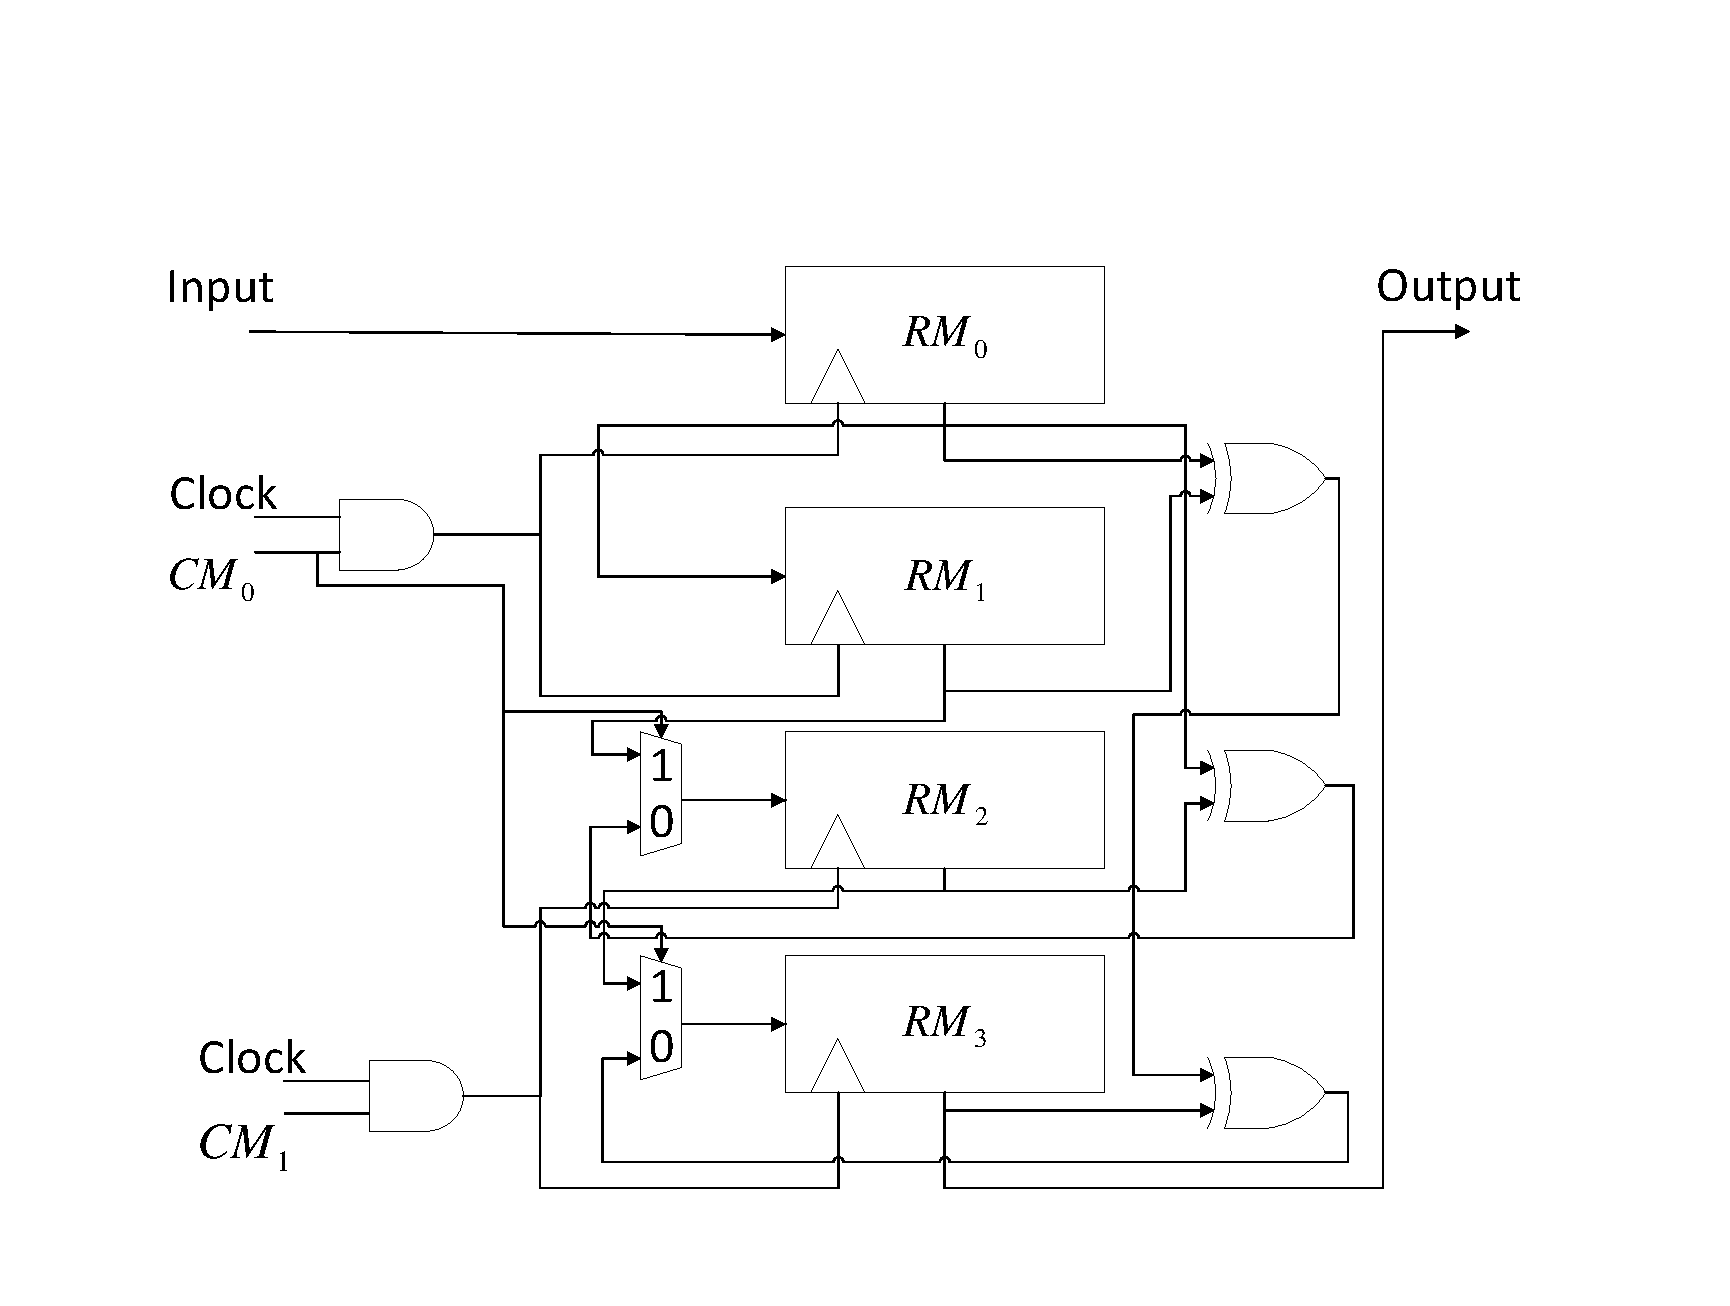
\includegraphics[width=\textwidth]{Mix-Columns.pdf}
    \caption{Serial Architecture of Mix-Columns with clock gating}\label{serial_mix_columns_fig}
\end{figure}

\begin{figure}[h]%   
    \centering
    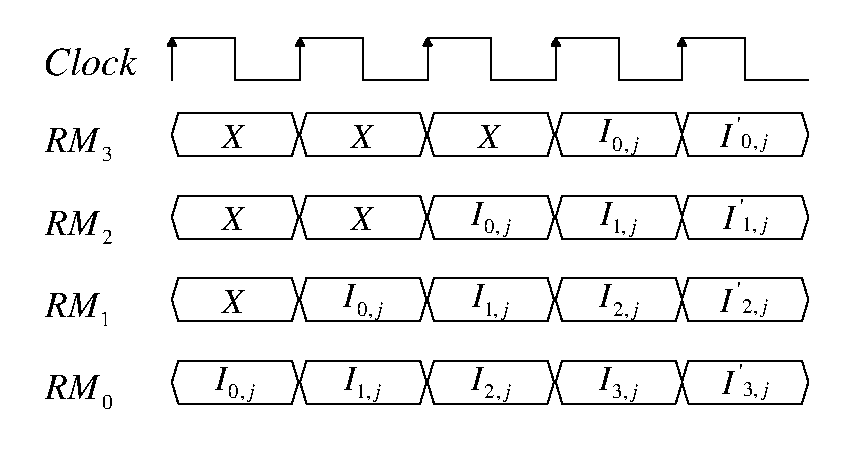
\includegraphics[width=\textwidth]{Mix-Columns-Times.pdf}
    \caption{Timing Diagram for the Serial Architecture of Mix-Columns }\label{serial_time_diagrm_mix_colunms}
\end{figure}

\subsubsection{Control Units}\label{subsubsec3}

The finite-state machine (FSM) of serial architecture is shown in Figure~\ref{serial_fsm_fig}.
The initial key and plaintext are stored in Key-Register and State-Register at the same time. After the Store, the key is expanded in Key Schedule.
In Mix Columns, one column of State-Register stores in the Mix Columns registers that take four clock cycles for execution Mix-Columns over one column.
In Add Key, the stored data in Mix Columns's registers are sent back to State-Register followed by XORing with keys and through the S-box component in another four clock cycles.
Permute executes in one clock cycle inside the State-Register.

\begin{figure}[h]%   
    \centering
    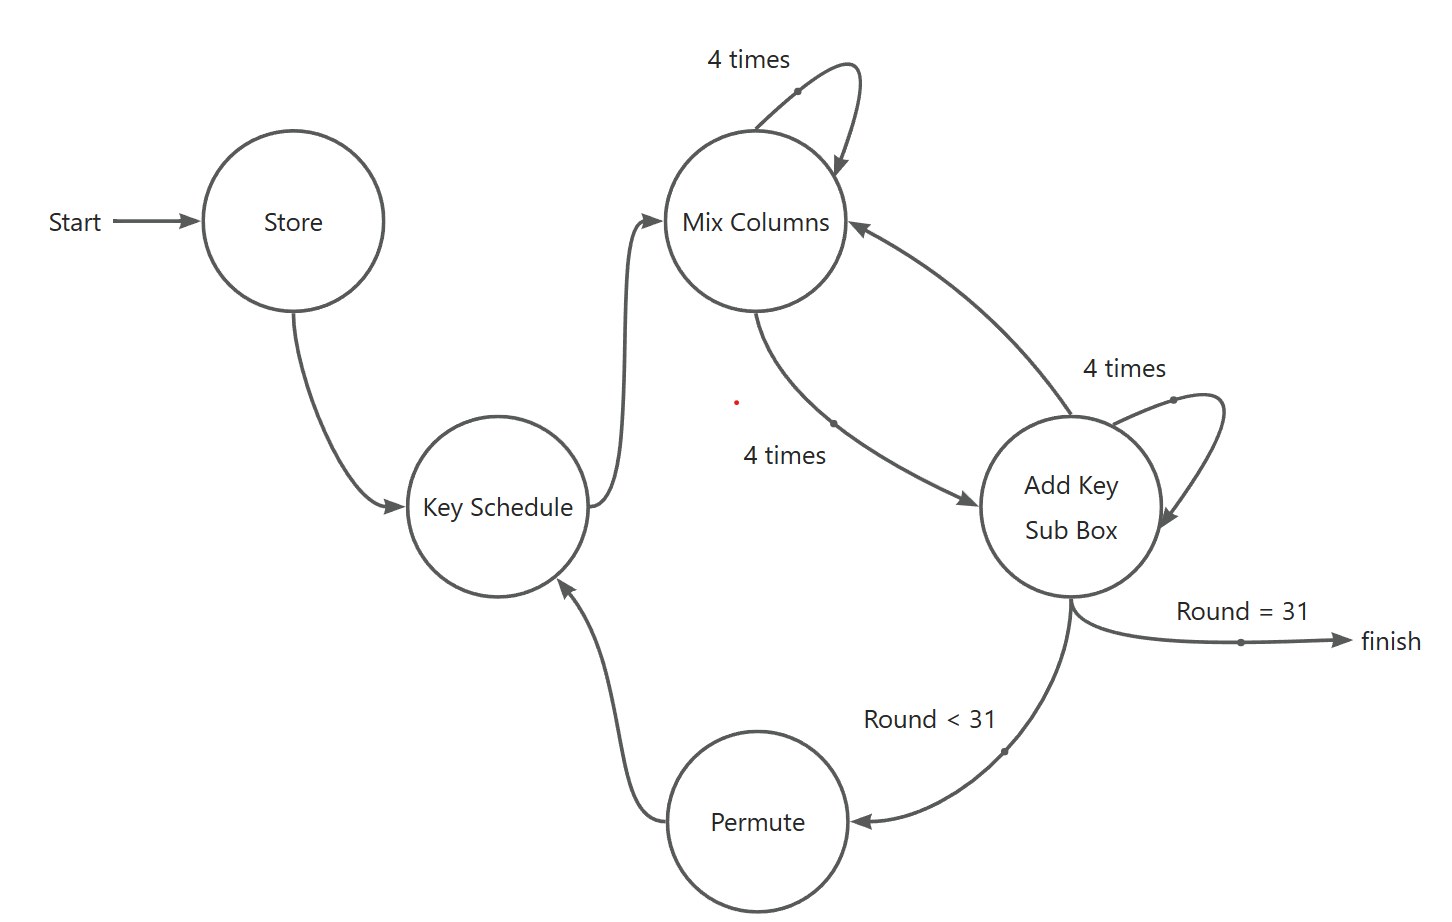
\includegraphics[width=\textwidth]{serial_fsm.png}
    \caption{Finite-state machine for Serial Architecture}\label{serial_fsm_fig}
\end{figure}

The dynamic power consumption of the encryption is reduced by employing clock gating, a technique discussed in \cite{shahbazi2020area}.
The clock gating is separately applied on State Register, Key Register and Mix Columns.
For instance, the most power consumption is saved during the Key Schedule phase; the clock of State Register and Mix Columns is disabled to save power because these two blocks are not used in the Key Schedule phase.
The timing diagram of the proposed design with the clock gating technique is shown in Figure~\ref{serial_time_diagrm}.

\begin{figure}[h]%   
    \centering
    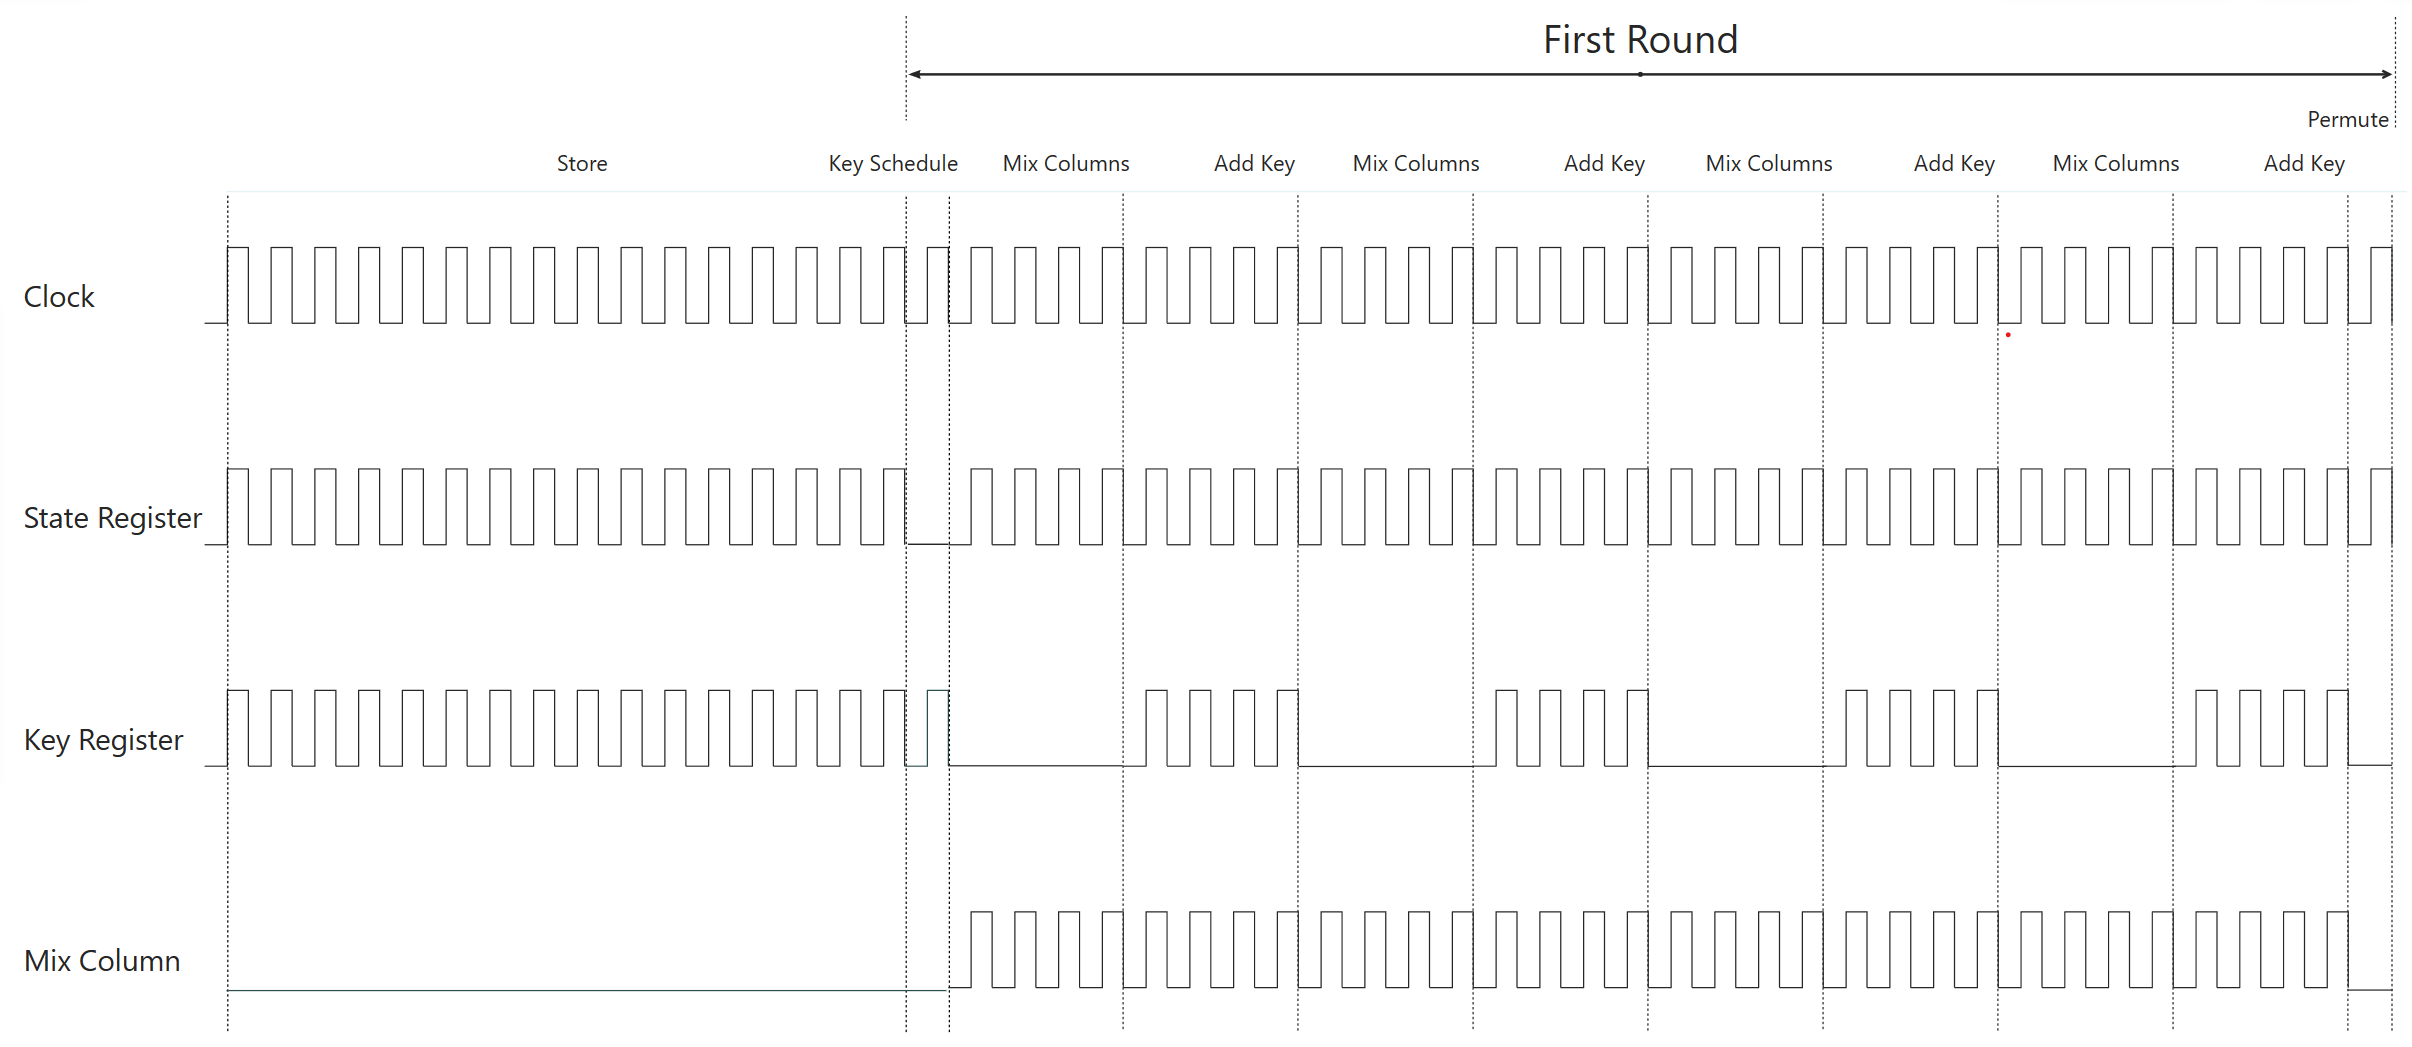
\includegraphics[width=\textwidth]{serial_time.png}
    \caption{Timing diagram for Serial Architecture}\label{serial_time_diagrm}
\end{figure}

\subsection{Loop Unrolled Architecture(A3)}\label{subsec3}

\section{Experimental Evaluation}\label{sec4}

In ASIC implementations, the gate equivalent (GE) is often used to evaluate the area consumption of a design. 
A single GE is equivalent to a two-input NAND gate. 
To calculate the area in GE, we divide the total area (in $\mu m^2$) by the area of a two-input NAND gate (also in $\mu m^2$). 
However, the number of GEs can vary based on the specific technology used, as discussed in \cite{mckay2016report}. 
For instance, the number of GEs for the same design will differ between UMC 180nm technology and TSMC 180nm technology. 
Therefore, GE is not suitable for comparing the area consumption of different designs on different technologies. 
In order to ensure a fair comparison, we evaluate the area consumption of the proposed designs using FPGA implementations, a method also utilized in \cite{mohajerani2020fpga}.

\subsection{Platform}\label{subsec4}

We implemented the proposed architectures on a Xilinx FPGA board using the ISE Design Suite 14.7 and Vivado v2023.2. 
We analyzed four different FPGA platforms: Spartan-3 (xc3s200-5ft256), Spartan-6 (xc6slx16-3csg324), Virtex-4 (xc4vlx25-12ff668), and Virtex-5 (xc5vlx50t-3ff1136) using the ISE Design Suite 14.7, a methodology also employed by \cite{lara2017lightweight}. 
For benchmarking on the latest FPGA, we used the Artix-7 (xc7a100tcsg324-1) platform with Vivado v2023.2, as done by \cite{mohajerani2020fpga}.


\subsection{Area}\label{subsec5}

We use the Area metric to evaluate the area consumption of the proposed designs, which includes components like flip-flops, LUTs, and slices. 
Given the different types of LUTs, such as LUT-4 and LUT-6, we use Spartan-3 and Virtex-4 for LUT-4, Spartan-6 and Virtex-5 for LUT-6, and Artix-7 for LUT-6. 
To ensure a fair comparison, we decided not to use the FPGA's embedded memory blocks by disabling the corresponding flags in the VHDL, as suggested in \cite{xilinx2022ultrafast}.

\subsection{Throughput}\label{subsec6}
We evaluate the performance of our proposed designs using the Throughput metric. 
This metric is assessed using three parameters: the maximum throughput rate, the throughput rate at 200MHz (following the method used by \cite{ghosh2017lightweight}), and the throughput rate per slice. 
The maximum throughput rate, calculated using Equation ~\ref{eq4}, represents the highest rate our designs can achieve. 
The throughput rate at 200MHz, calculated using Equation ~\ref{eq5}, shows the rate achievable when the clock frequency is set to 200MHz. 
Finally, the throughput rate per slice, calculated by dividing the throughput rate by the number of slices (Equation ~\ref{eq6}), provides a measure of efficiency. 
In these calculations, the Plaintext Size is 64-bit, Latency refers to the number of clock cycles required to encrypt a single block, and Slices refers to the number of slices used by the design.

\begin{equation}
    Maximum Throughput(Thr) = \frac{Maximum Frequency \times Plaintext Size}{Latency} 
    \label{eq4}
\end{equation}

\begin{equation}
    Throughput_{@200MHz}(Thr^*) = \frac{200MHz \times Plaintext Size}{Latency} 
    \label{eq5}
\end{equation}

\begin{equation}
    ThroughputPerSlice = \frac{Throughput_{@200MHz}(Thr^*)}{Slices} 
    \label{eq6}
\end{equation}

\section{Results}\label{sec5}

In terms of area, the consumption of each component of the algorithm is shown in Table~\ref{area_cost_round_based}.
The larger part of the footprint is the intermediate register state and the non-linear component S-box.
In terms of throughput, The critical path is from the control register to the intermediate value register state, which has a delay of 5.2ns. the calculated maximum throughput rate is 382Mbit/s.

\begin{table}[h]
    \caption{Area consumption of Round based design}\label{area_cost_round_based}%
    \begin{tabular*}{\textwidth}{@{\extracolsep\fill}lcccccc}
        \toprule
        &LUT&	FF&	Slice                                \\
        \midrule
        Key Schedule &	64&	0&	22                           \\
        Round Constant&	2&	7&	2 \\
        S-box * 4&	8&	0&	4                             \\
        Round (include  S-box * 16)&	84&	0&	28                        \\
        All (include control)&	182&	144&	56                     \\
        \botrule
    \end{tabular*}
\end{table}

\section{Conclusion}\label{sec6}

\bibliography{sn-bibliography}% common bib file
%% if required, the content of .bbl file can be included here once bbl is generated
%%\input sn-article.bbl

\end{document}
